\documentclass{template/openetcs_report}
% Use the option "nocc" if the document is not licensed under Creative Commons
%\documentclass[nocc]{template/openetcs_article}
\usepackage{lipsum,url}
\graphicspath{{./template/}{.}{./images/}}

\begin{document}
\frontmatter
\project{openETCS}

%Please do not change anything above this line
%============================
% The document metadata is defined below

%assign a report number here
\reportnum{OETCS/WP4/D4.2.3V02}

%define your workpackage here
\wp{Work-Package 4: ``Validation \& Verification Strategy''}

%set a title here
\title{openETCS Hazard and Risk Analysis Methodology}

%set a subtitle here
\subtitle{Guideline for the safety related activities in an openETCS Onboard Unit development}

%set the date of the report here
\date{March 2014} %\\ Revised March 2013}

%define a list of authors and their affiliation here

\author{Jan Welte}

\affiliation{Technische Universität Braunschweig\\
  Institute for Traffic Safety and Automation Engineering\\
  Langer Kamp 8\\
  38106 Braunschweig, Germany\\
  eMail: openetcs@iva.ing.tu-bs.de \\
  WebSite: www.iva.ing.tu-bs.de}

%add yourself as author, if you contributed to the document



% define the coverart
\coverart[width=350pt]{openETCS_EUPL}

%define the type of report
\reporttype{Output Document}


\begin{abstract}
This document presents an overview about the main activities performed during the OpenETCS development process to identify hazards inside the openETCS software and to assess the risk resulting from these hazards. Thereby, a consistent methodology is derived, which connects the hazard and risk analysis for the system and subsystems from which potential hazards and corresponding risks will be derived with methods to identify and enforce  to ensure the overall quality during the design of all safety related parts of the system. Overall, the safety plan will guarantee that the safety design activities required in D2.6 are covered and all safety requirements are fulfilled. 
\end{abstract}

%=============================
%Do not change the next three lines
\maketitle
\tableofcontents
\listoffiguresandtables
\newpage
%=============================

\chapter{Document Control}

\begin{tabular}{|p{4.4cm}|p{8.7cm}|}
\hline
\multicolumn{2}{|c|}{Document information} \\
\hline
Work Package &  WP4  \\
Deliverable ID or doc. ref. & D4.2\\
\hline
Document title & openETCS Safety Plan\\
Document version & 00.20 \\
Document authors (org.)  & Jan Welte (TU-BS)\\
\hline
\end{tabular}

\begin{tabular}{|p{4.4cm}|p{8.7cm}|}
\hline
\multicolumn{2}{|c|}{Review information} \\
\hline
Last version reviewed & -- \\
\hline
Main reviewers & -- \\
\hline
\end{tabular}

\begin{tabular}{|p{2.2cm}|p{4cm}|p{4cm}|p{2cm}|}
\hline
\multicolumn{4}{|c|}{Approbation} \\
\hline
  &  Name & Role & Date   \\
\hline  
Written by    &  Jan Welte & WP4-T4.4 Task Leader  &  October 2013\\
\hline
Approved by & -- & -- & \\
\hline
\end{tabular}

\begin{tabular}{|p{2.2cm}|p{2cm}|p{3cm}|p{5cm}|}
\hline
\multicolumn{4}{|c|}{Document evolution} \\
\hline
00.01 & 01/10/2013 & Jan Welte &  Document creation \\
\hline
Version &  Date & Author(s) & Justification  \\
\hline  
00.1 & 28/01/2014 & Jan Welte &  Extended Introduction  \\
00.2 & 14/03/2014 & Jan Welte &  Reword document structure to incorporate review comments from internal assessment \\
\hline  
\end{tabular}
\newpage

% The actual document starts below this line
%=============================

\mainmatter

\chapter{Introduction}
\label{sec:introduction}

During system development the system limits and components have to be established before the necessary steps can be taken to ensure that the system behavior is not unsafe. In this context safety is understood as protecting the environment from hazards coming from the system as distinguished from security which covers protecting the system itself from hazards coming from the outside. Respectively, safety and security are comparative terms which have to be specified in context of the system for which they shall be proven. The standards for system development like EN 50126, EN 50128 and EN 50129 provide only guidelines how safety for a system shall be determined and assured by providing certain management principles and methods for the respective system development. As the openETCS project is related to a number of different system definitions like the overall railway system, the on-board unit, the Kernel software and the development tool chain different safety aspects have to be taken in consideration. Only a small number of these can actually be determined in the openETCS context alone.

\section{Purpose}
\label{sec:purpose}

The safety plan is part of the overall safety process which is "the series of procedures that are followed to enable all safety requirements of a product to be identified and met" \cite{EN50129}. To ensure that the safety process is implemented in a proper way the EN 50129 requires a safety management which is consistent process for RAMS presented in the EN 50126. 

The purpose of the safety plan is to show in details how the safety requirements will be implemented over the development process. To do this the plan has to present the management structure, all related activities and documentations over the life-cycle, as well as the approval mile-stones and review requirements. As the product life-cycle is an ongoing process and, specifically in a project like openETCS, iterative changes are taking place, the safety plan has to be updated to assess the respective safety effects. Thereby, the safety plan will also include the plan for the safety case, which itself is the final assessment document to demonstrate the actual product compliance with all specified safety requirements which have been implemented according to the safety plan.

As the movement characteristics of a train set specific limits in which a driver alone is able to avoid derailment or any kind of collisions railway signaling and protection systems have been developed to ensure safe train movements. Respectively, the mayor parts of a train control system like ETCS include functionalities which shall guarantee that the overall railway system does not get in a hazardous situation.

Since the openETCS project does not produce a specific train borne on-board unit the openETCS safety plan, will not cover all specific software and hardware aspects. The focus is mainly on the EVC kernel functionality and only partially on further real time and hardware/software integration aspects. However, this safety plan shall at least cover the safety process needed to ensure that the openETCS software development can be extended to become the functional basis for a complete on-board unit development. 

\section{Document Structure}
\label{sec:document-structure}

As the openETCS software development process and the respective tool chain a used in an iterative process this version of the safety plan is also only one iteration step. As the design selectivities and the use of tools proceed further more details concerning the hazard identification methods, safety verification and validation principals and their corresponding result documentation will be added to this document. So far the version 1.0 of the safety plan will only cover the overall safety process and it general activities as well as the safety management activities which will create the safety plan as the final documentation document. Details are only presented for the hazard identification and evaluation method, as well as for the argumentation structure management method. All detailed activities concerning verification and validation of different safety requirements are closely connected to the V\&V plan and all activities described there. 

As safety is a term which is used in different context and therefore interpreted differently depending on the used reference system, the following section \ref{sec:Background} presents the principal concept and terminology on which the following safety process is founded \cite{Schnieder 2013}. These section shall present and clarify the underlying understanding of safety as it in standards EN 50126, EN 50128 and EN 50129 for railway system development. Thereby, it is important to state more precisely the relation between quality and safety for software as this is the core aspect for the openETCS development.

\section{Background Information}
\label{sec:Background}

In the context of railway system development the EN 5012X and the ISO 900X standards are closely connected. Respectively, the terms safety and quality and related terms as reliability, maintainability, availability, usability and security are often used together. For example the EN 50129 names evidence of quality and safety management as conditions for a safety acceptance. The following sections shall give a common definition for all this aspects, which are required in a CENELEC confirm development process. 

\subsection{Quality}

The ISO 9000 defines quality as "degree to which a set of inherent characteristics fulfills requirements" \cite{ISO9000}, which clearly shows a more objective view as the EN 50129, which defines quality as "a user perception of the attributes of a product" \cite{EN50129}. As for system development the given requirements always present the objective against which the system has to be measured this definition is consistent with the definition of verification and validation as it is presented in the EN 50128 and the openETCS V\&V plan.

Depending on the respective field of application specific standards further specify the characteristics which shall be taken in account to establish quality. The EN 50126 as primary standard for railway applications gives RAMS as the major contributor for the quality of service. 

\subsection{RAMS}



\begin{figure}[htbp]
\centering
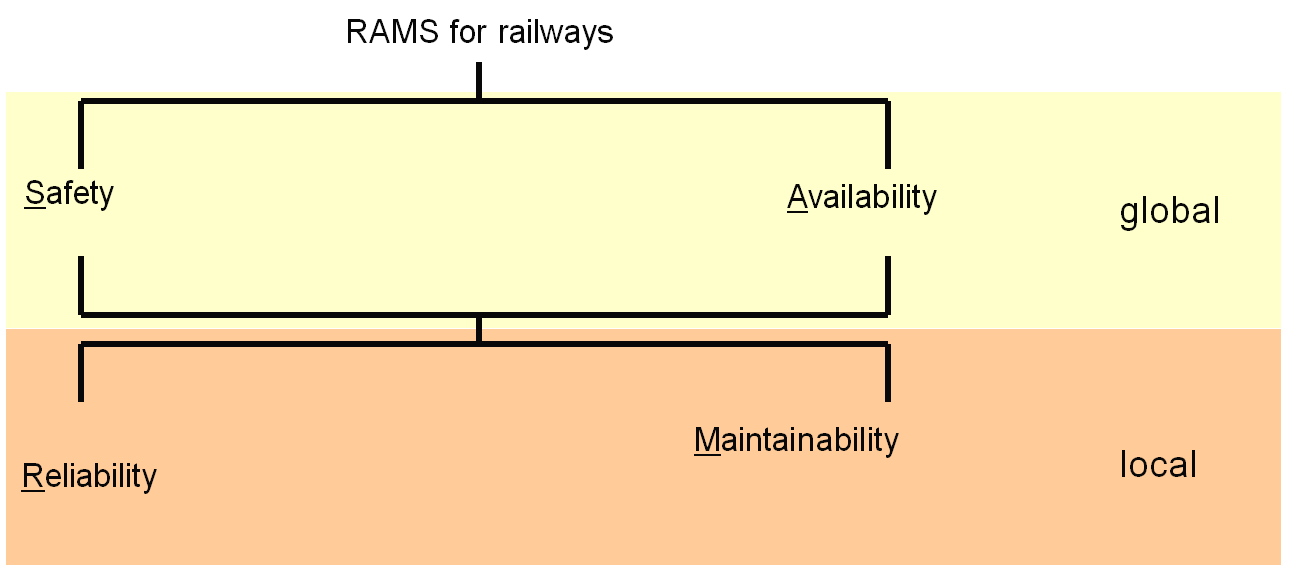
\includegraphics[width=0.7\linewidth]{images/bld_RAMS-Railway-50126}
\caption{RAMS for Railway elements and their relations \cite{Schnieder.2013}}
\label{fig:RAMS-EN50126}
\end{figure}


\begin{figure}[htbp]
\centering
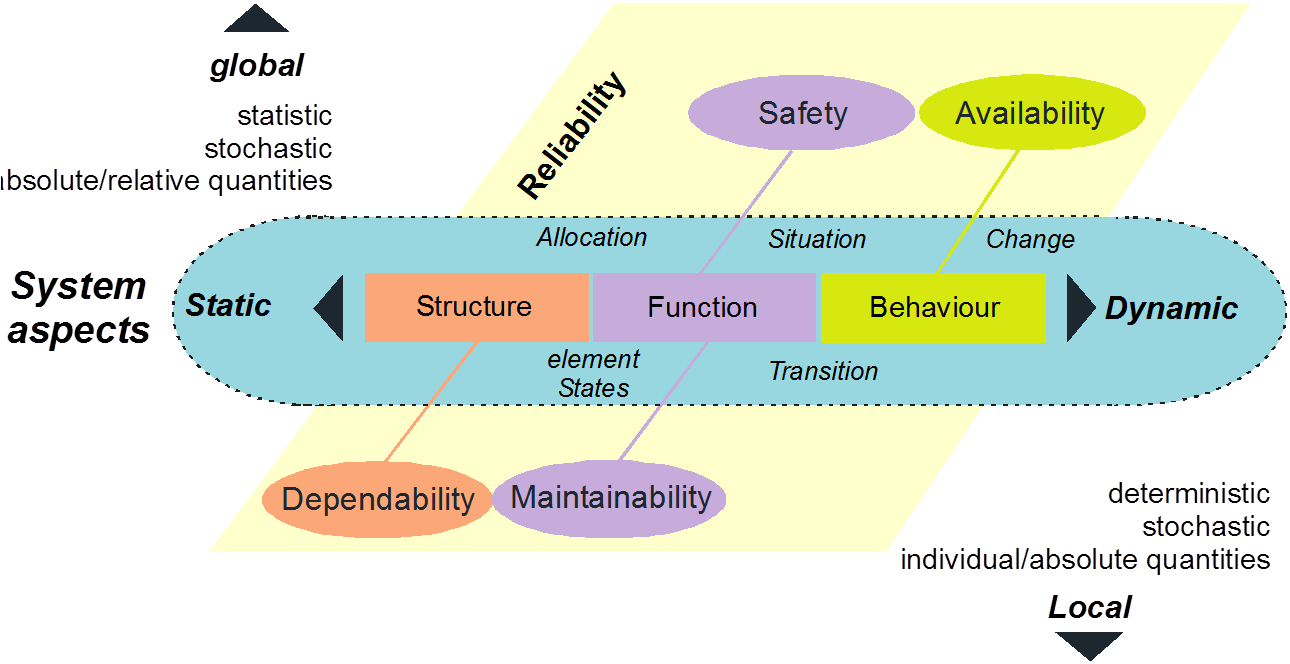
\includegraphics[width=0.7\linewidth]{images/bld_Reliability-system-characteristics}
\caption{Systems Characteristics and their relations to RAMS in Railways \cite{Schnieder.2013}}
\label{fig:Reliability-RAMS}
\end{figure}

\subsection{Software Quality}


\subsection{Safety}



\subsection{Probabilistic Safety Concept}

\paragraph{Risk}

The EN50128 standard defines safety as the ``freedom from unacceptable levels of risk of harm to people" \cite{EN50128:2011}, which shows that the safety approach required by the CENELEC standards is risk-based. As the risk is defined as the ``combination of the rate of occurrence of accidents and incidents resulting in harm (caused by a hazard) and the degree of severity  of that harm" \cite{EN50128:2011} this approach is based on a probabilistic understanding of event occurrence. The overall relations between all these safety-related terms used to define the safety properties, characteristics and quantities are outlined by the Risk-Genesis-Model of Schnieder, which is shown in the following figure \ref{fig:Risiko-Genese-Modell-eng}.

\begin{figure}[htbp]
\centering
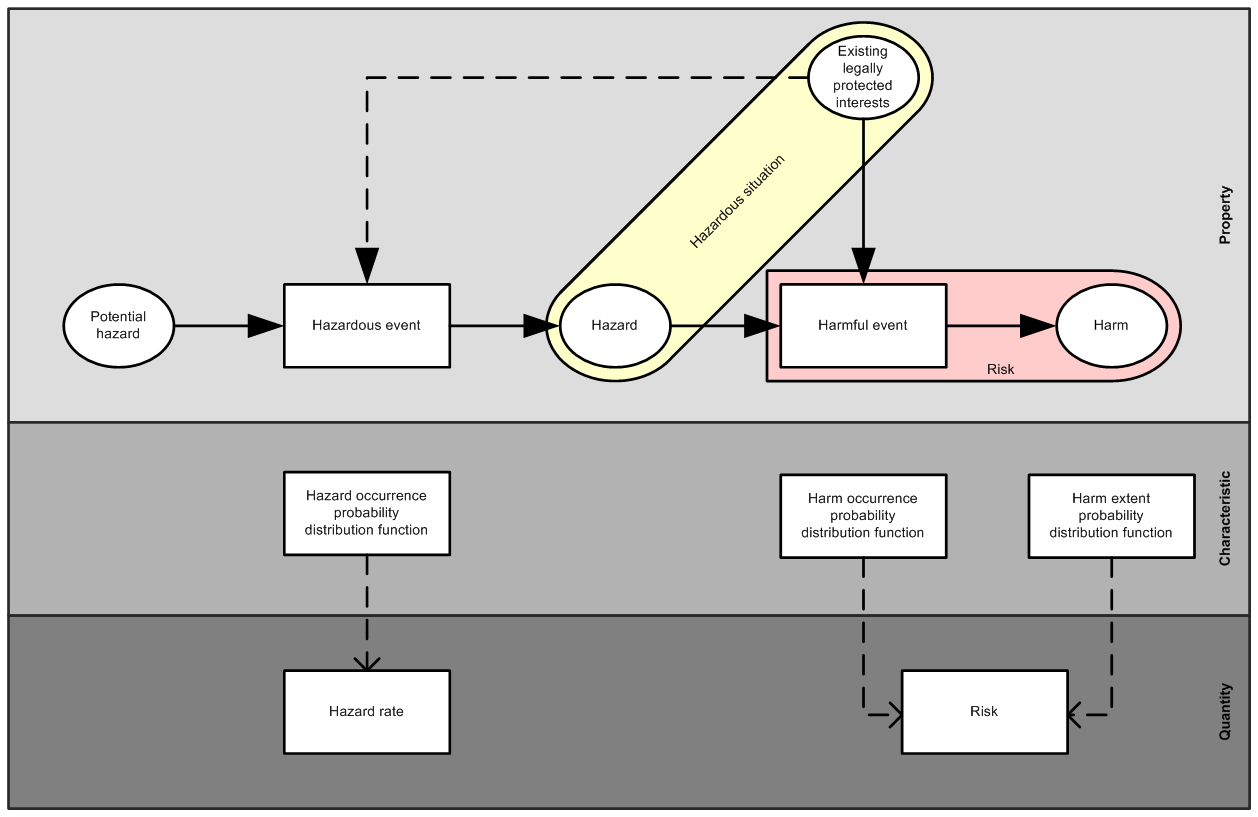
\includegraphics[width=0.7\linewidth]{bld_2013-06-19_Risiko-Genese-Modell-eng-2-0_jw}
\caption{Risk-Genesis-Model showing the relations between the safety-related terms \cite{Schnieder.2010}}
\label{fig:Risiko-Genese-Modell-eng}
\end{figure}

This demonstrates that the first step is to define the system properties, specifically identifying the harms and their related hazardous situations. This has to be performed during a system hazard analysis. Afterwards the respective properties have to be determined by assessing the risk concerning the identified hazards. Based on this work safety integrity levels can be assigned to all system functionalities which are then allocated during the design to certain parts of the operational equipment. As this work is closely related to all design decisions, it has to be done iteratively for all abstraction levels during the system design. 

\begin{figure}[htbp]
\centering
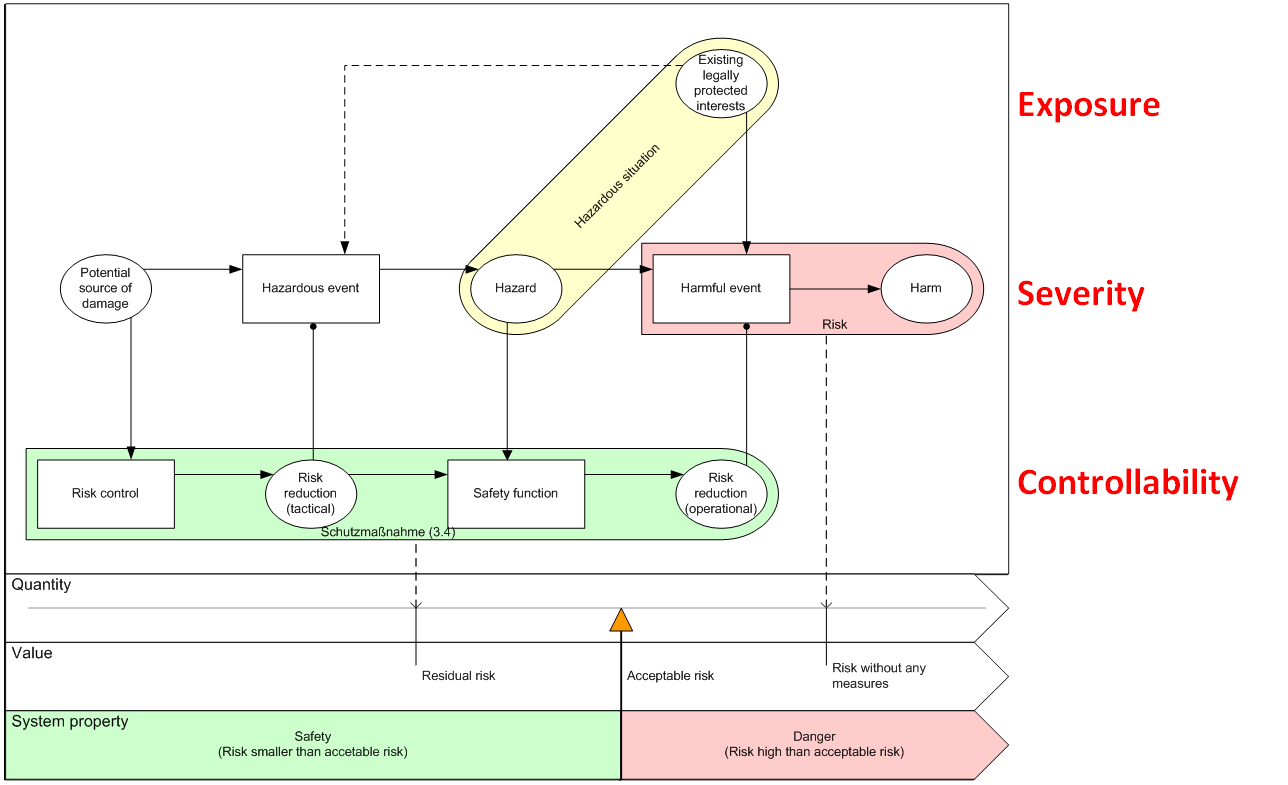
\includegraphics[width=0.7\linewidth]{bld_2013-06-19_Risk-control-modell_1-0_jw}
\caption{Risk control process \cite{Schnieder.2013}}
\label{fig:Risk-control-modell-eng}
\end{figure}

\paragraph{Safety Integrity Level}

The safety integrity level represented the acceptable risk for every part of the system. The risk control process as it is presented in figure \ref{fig:Risk-control-modell-eng} is then performed to ensure that the safety integrity levels are reach by every part of the system.

Since software itself does not fails in the way technical equipment does the specific software safety integrity level represent a qualitative measure with respect to the required degree of correctness for the software functionality than a qualitative value for the likelihood of failing. To reach the needed degree of correctness for the software various design, verification and validation methods are required corresponding to the assigned software safety integrity level. This process leads to safety requirements which have to be implemented in the software design as well as verified and validated. Respectively the EN50126 describes the safety design process as a series of safety tasks for each life cycle phase. This task are related to a number of safety artifacts which are created, used and adapted over time through the different safety design activities.


\subsection{Safety Case}

The EN 50129 states that evidence of quality management, safety management, as well as functional and technical safety have to be provided for safety acceptance. The safety case shall be the structured safety justification document demonstrating that these conditions have been satisfied.
Therefore, the British Ministry of Defence defines a safety case as “a structured argument, supported by a body of evidence that provides a compelling, comprehensible and valid case that a system is safe for a given application in a given environment.”\cite{MinistryofDefence.2005} This definition emphasizes the distinction between the “argumentation” and the “evidences”, which corresponds to the distinction between rules coming from the legal requirements and facts resulting from the actual working process. This clear distinction between the safety argumentation and the evidences helps to structure the safety case and improvement of the discussions with the legal authorities.\cite{Müller.2010}

%\subsection{Safety Glossary}

%\textbf{Added via the glossary documentation process for openETCS}

\chapter{Document Evolution}

This document will be further specified with the progress of the design process to update and detail the corresponding hazard and risk analysis methods. This specifically reference to the refinement of safety properties on different modeling levels and their corresponding verification and validation methods. All resulting changes and additional safety activities have to be maintained according to the EN~50128 and document according to the overall safety case process. 

The openETCS development plan presented in chapter \ref{development-process} is based on the available information in the Quality Assurance Plan and from WP 2 D2.3 and D2.4. As the development methods and processes are still evolving this document has to be adopted accordingly.

Concrete methods to verify and validate safety relevant properties derived from the hazard control methods descriped in this document, will be specified in the Verification and Validation plan. Also the tools used to support those activities will be detailed in this plan.

\chapter{OpenETCS Development process}

The main products of the openETCS project will be the OpenETCS specification model used to generate the OpenETCs on-board software and the OpenETCS tools chain development, which is used to formalizes the ERA Specifications for ETCS, generate the Software Code and perform verification and validation activities. Both parts have their own development process, but the focus focus hazard and risk analysis and the safety case shall be on the software development process. The openETCS tool chain shall only be considered with respect to its role in the software development process as the tool qualification is mainly out of this project.
The safety related activities 

\section{Formalization and software development}

The software development in the OpenETCS project shall be performed as an open, model-based, agile Software development. The respective combination of methods used during the development process shall comply with a SIL 4 development process according to EN 50128 for which the requirements are analyzed and shown in detail in D2.2. The overall openETCS Software development process presenting the development principals how the on-board unit requirements for ETCS shall be formalized first in a semi-formal SysML architecture model and afterwards in a detail formal SCADE behavior model, which is the basis for the automatic source code generation, are outlined in WP 2 D2.3 and D2.4. 

The detailed principals and phases of this development process are presented in the Quality Assurance Plan. As this development process and the supporting tools are still evolves the detailed development description has to be updated as the project continues. 


\begin{tabular}{|p{1cm}|p{2cm}|p{8cm}|p{3cm}|}
\hline \textbf{Phase} & \textbf{Name} & \textbf{Description} & \textbf{Main Tool component} \\ 
\hline P1 & Software Requirement Phase & Requirement input documents converted to a ReqIF format and informally analyses. The analysis specifies relationships between requirements and revises parts of the requirements to obtain a detail and atomic abstraction level usable for moralization. To support thus the requirements are categorized and grouped. & ProR \\ 
\hline P2 & Software Architecture Modeling Phase & Building a SysML based on the informal analysis using the categorization of requirements. The architecture model focuses on functional blocks and data flows. & SysML Papyrus \\ 
\hline P3 & Software Behavior Modeling Phase & Building the SCADE model for the separated basic functional blocks. The SCADE model describes the detailed behavior for the function using the data flows. & SCADE \\ 
\hline P4 & Formal Validation phase & Using test models and model checking techniques, to validate the correct model behavior.  & Various \\ 
\hline 
\end{tabular} 


\section{Safety Interfaces}

\textit{Clear description of the interfaces to the process providing inputs for safety and using the Safety results. Specific describing the applied iterations.}

\subsection{Specific Interfaces to the Design Process}

\subsection{Interface to Quality Management}

\subsection{Interface to Verification}

\subsection{Interface to Validation}


\textit{Short description for the needed documentation}



\chapter{Hazard and Risk Analysis}



\section{General ETCS Safety Principals}

\textit{This section shall present as short description of all safety principals used for the overall safety strategy.}



\section{OpenETCS Activities}


\begin{figure}[h]
\centering
\includegraphics[width=0.7\linewidth]{./images/WholeSafetyProcess}
\caption[Overall safety process]{Overall safety process}
\label{fig:SafetyProcess}
\end{figure}

\textit{Process description has to be updated with the latest work. Cooperation between Cyril, Merlin and Jan}

\subsection{OpenETCS safety design process}

The presented CENELEC standard safety artifacts and activities are always related to the overall system development. Since the openETCS development process just describes the development of the on-board unit software for ETCS additional system informations are needed for the openETCS safety design process. These are mainly the following two parts of the CCS TSI:

\begin{itemize}
\item UNISIG SUBSET-026	System Requirements Specification 	(Version 3.3.0)
\item UNISIG SUBSET-091 Safety Requirements for the Technical Interoperability of ETCS in Levels 1 and 2 	(Version 3.2.0)
\end{itemize}

In relation to SUBSET-91 further documents should be considered:

\begin{itemize}
\item Part of TSI Annex A
	\begin{itemize}
	\item SUBSET-036
	\item SUBSET-037
	\item SUBSET-040
	\item SUBSET-041
	\item SUBSET-098
	\end{itemize}
	
\item Not part of TSI Annex A
	\begin{itemize}
	\item SUBSET-039
	\item SUBSET-078
	\item SUBSET-079
	\item SUBSET-080
	\item SUBSET-081
	\item SUBSET-088
	\end{itemize}
\end{itemize}

From these documents the Preliminary Hazard Analysis and the System Safety Goals have to be derived which are needed as the starting point for the openETCS safety design process. Based on these information a subsystem hazard and risk analysis for the openETCS scope can be performed which set-up the openETCS hazard log. Based on these results the openETCS safety requirements will be specified, which are then further developed to functional requirements. During the development these requirements are adopted if necessary for the different abstraction levels from the high level model down to the source code. This is done using corresponding safety backlogs, which are the reference for the safety requirement verification. Altogether the source code has to be validated against all safety requirements to demonstrated, that software faults can not cause any harm. The safety case has to present all needed documentation.
 
The main task of the openETCS safety design process and the interactions with the design process are shown in figure \ref{fig:WholeSafetyProcess}.

\begin{figure}[htbp]
\centering
\includegraphics[width=0.8\linewidth]{WholeSafetyProcess}
\caption{OpenETCS Safety Design Process}
\label{fig:WholeSafetyProcess}
\end{figure}

The openETCS safety design process will be specified more detailed in the safety plan. Correspondingly, the main safety artifacts and safety design activities which have to be handled during the openETCS safety design process are shown in table \ref{tab:openETCS-Safety-artifacts} and \ref{tab:openETCS-Safety-activities}.

% Table generated by Excel2LaTeX from sheet 'Artifact Categorization'
\begin{table}[htbp]
  \centering
  \caption{Main openETCS safety design process artifacts}
    \begin{tabular}{r|p{8cm}|p{4cm}}
    \textbf{Abbreviation} & \textbf{Safety Artifact} & \textbf{Degree of Formalisation}\\
    \hline
    Safety Req & Safety Requirements: list of all requirements which have to be respected during the system development to reach the safety goals & Informal/ Semi-Formal / Formal \\
    HL    & Hazard Log: List of identified hazards and its associated risk classification as well as information concerning the risk control & Informal \\
    SP    & Safety Plan: Document which specifies all activities, resources and events to ensure that the source code will satisfy all relevant safety requirements & Informal \\
    SC    & Safety Case: Documentation which demonstrates that the used development process and the resulting source code fulfil all safety requirements & Informal \\
    CSB   & Code Safety Backlog: list of requirements/ properties to be implemented inside the dM derived from  the HL (and the dMSB) & Semi-Formal/ Strictly-Formal \\
    dMSB  & Detailed Model Safety Backlog: list of requirements/ properties to be implemented inside the dM derived from the HL (and  the hLSB) & Semi-Formal/ Strictly-Formal \\
    hLSB  & High Level Safety Backlog: list of requirements/ properties to be implemented inside the hM derived from the HL & Informal/ Semi-Formal \\
    \end{tabular}%
  \label{tab:openETCS-Safety-artifacts}%
\end{table}%

\begin{table}[htbp]
  \centering
  \caption{Main openETCS safety design process activities}
    \begin{tabular}{p{4cm}|p{6cm}|p{4cm}} 
 \textbf{Safety Design Activity} & \textbf{Input Artifact(s)} & \textbf{Output Artifact(s)}  \\ \hline
 Establish Safety Plan & QA-Plan + Project documentation (FPP, …) & Safety Plan \\
 Preliminary Hazard Analysis (PHA) & Mainly SUBSET-91(+SUBSET-88) &  Safety Goals + Safety Acceptance Criteria +  PHA report\\ 
 Sub-System Hazard and Risk Analysis (SSHA) & Safety Goals and Acceptance Criteria + SSRS + additional design and architecture specification + additional user constraints  & Hazard Log (incl. Hazards and Safety Functions) \\ 
  Specification of Sub-System Safety Requirements & SUBSET-26 + SUBSET-91 + Hazard Log  & Safety Requirement Specifications \\ 
 Update Hazard Log and corresponding Sub-System Safety Requirements & Verification Reports + Test Cases & Hazard Log + Sub-System Safety Requirements \\
 Specify model specific Requirements & SSRS + Safety Requirement Specification & Safety Plan + Model Backlogs\\
 Verify Safety Requirements & Models + Safety Requirements + Model Backlogs & Verification Report + Verification report \\
 Validate Safety Requirements & Source Code + Safety Requirements & Validation Report + Validation report \\
 Establish Safety Case & V and V Plan + Safety Plan + all requirements and specifications + V and V Reports & Safety Case \\ 
 
\end{tabular}  
  \label{tab:openETCS-Safety-activities}%
\end{table}%

The safety design process and the resulting documentation constitute the main documents for the system approval, as it is required by European and national law to do everything reasonable expectable to prevent harm. Accordingly the CENELEC standards build the common technical rules for the development process. The Common Safety Methods present a concept based on the EN50126 how the risk evaluation and management has to be performed. 

Therefore the main references concerning the safety design process are the CENELEC standards, mainly the EN50126 on how the safety aspects have to be handled as part of the RAMS management over the development process. The overall risk evaluation concept is also defined at this point. The specific concerning the safety case preparations are defined in the EN50129 including the Safety Integrity Level concept. 

Therefore the overall safety management process has to be followed during the openETCS project, as far as it is concerning the scope of openETCS. Therefore the following table \ref{tab:Safety Process Requirements} presents a first list of relevant requirements:

\begin{table}[htbp]
  \centering
  \caption{CENELEC Safety Process Requirements}
    \begin{tabular}{r|r|r}
    Standard & Section & Titel \\
    \hline
     EN 50126 & 4 & Railway RAMS  \\ 
    EN 50126 & 6 & RAMS lifecycle \\
     EN 50128 & Table A.3 & Software Error Effect Analysis\\
    EN 50129 & 5.3 & Evidence of safety management \\
    EN 50129 & Annex A & Safety Integrity Levels \\
    EN 50129 & Annex B & Detailed technical requirements \\
    \end{tabular}%
  \label{tab:Safety Process Requirements}%
\end{table}%




\subsection{Safety artifacts}

\textit{Process description has to be updated with the latest work. Cooperation between Cyril, Merlin and Jan}

Since all safety design activities are based on the system development activities all system design artifacts are part of the safety design process. Therefore, the following design artifacts of the CENELEC standard development process build the basis for all safety artifacts:

\begin{itemize}
\item System Concept
\item System Requirements Specification
\item Software Requirement Specification
\item Software Architecture Specification
\item Software Design Specification
\item Software Module Design Specification
\item Software Source Code
\end{itemize}

The main safety artifacts are those which are set-up to build the reference for the safety-related aspect during the system development, which are continuously evolved during the design phases. Correspondingly the safety design process has to create artifacts to demonstrated that all safety and quality-related requirements included in the system design. Respectively the following artifacts are created during the safety design process:

\begin{itemize}
\item System Safety Plan
\item Software Quality Assurance Plan
\item Hazard Log
\item System Safety Requirement Specification
\item Safety Case
\end{itemize} 

This artifacts have to be managed over the development process. Since all safety requirement have to be verified and validated there is likewise a close to all Test and Validation Reports.

\subsection{Safety design activities}
\label{safetyactivities}

\textit{Process description has to be updated with the latest work. Cooperation between Cyril, Merlin and Jan}


The safety design activities set-up or evolve the safety artifacts in relation to the different design artifacts. The following safety design activities are required according to the EN 50128:

\begin{itemize}
\item Preliminary Hazard Analysis
\item Establish Safety Plan
\item System Hazard and Risk Analysis
\item Risk Assessment
\item Specification of System Safety Requirements
\item Define Safety Related Functional Requirements
\item Specify Sub-System and Component Safety requirements
\item Implement Safety Plan
\item Verify System, Sub-System and Component Safety requirements
\item Validate System Safety Requirements
\item Establish Safety Case
\end{itemize}

Overall the safety design activities have to be performed in close relation to the overall verification and validation activities as these have to verify and validate all safety requirements and their results become part of the safety plan.


\section{Safety design process supporting tools}

Supporting software tools are needed to handle the safety artifacts and to some degree to more efficiently perform the safety design activities. As some safety artifacts like the safety requirement specifications and the safety backlogs are closely related to design artifacts the same tools can be used. Especially all requirements should be handled by one tool to ensure full traceability and provide one main interface for the verification and validation activities.

Depending on the methods used for hazard and risk analysis appropriate tools are needed to perform the analysis, collect the hazards and associated risks in the hazard log and to evaluated possible risk control measures. Thereby, traceability has to be guaranteed between all activities.

Since the safety plan and safety case provide the basis for the safety approval the tools used to generated these artifacts should help to generate a consistent argumentation and efficiently collect the data needed to provide evidence. Respectively, interfaces to manage documents and automatically generate reports would be helpful functionalities.


\section{Proof of concept}
\label{sec:Proofofconcept}

The VnV Level 1 activities try to implement the overall safety strategy on parts of the benchmark modelling results to establish details for artifact relations, traceability between different artifacts and tool use. Therefore the following benchmark models are used as exemplary design artifacts:

\begin{itemize}
\item SysML model Papyrus by CEA and All4tec

\item Fraunhofer

\item Scade model by Siemens
\end{itemize}



\subsubsection{Hazardous Events}

Based on the 
\begin{itemize}
\item [a.] KERNEL-6  Manage communication session failure - Related to model of Subset 26 §3.5.3 Establishing a communication session
\item [b.] KERNEL-9  Speed calculation underestimates train speed (or KERNEL-25  Incorrect traction/braking model (Acceleration only)) - Related to model of Subset 26 §3.13 Braking curves
\item [c.] KERNEL-19  Failure of train trip supervision in OS, LS and FS - Related to model of Subset 26 §5.9 Procedure On-Sight
\end{itemize}



\chapter{OpenETCS Safety Case}

If the openETCS specification model and the generated on-board software shall be used in operation sufficient documentation is needed to demonstrate the used quality and safety management and their methods according to CENELEC standards, so that all potential implementers know which steps have to be performed by them to provide a safe product. 
One of the resulting objectives of the openETCS project is to identify an efficient way for the safety case process and to develop improvement strategies to reach certification at various National Safety Authorities thus reducing time and money  in industry for the ETCS development by avoiding unnecessary or redundant procedures. 



\section{Structure}

Starting from a set of requirements, the strategy to demonstrate the safety of a product is to be developed and graphically described (see figure 1). In general, the fulfilment of each requirement will be shown by a tree of argumentation. The leaves of these trees specify the corresponding evidences (e.g. test results or analysis results). These evidences have to be documented and the corresponding documents accrue during the corresponding phases of the CENELEC development process described in the EN 50126.
It turned out that such graphical argumentation structures ease the discussions with legal authorities as they understand the essence of the argumentation strategy in a very short time. In addition, through referencing the corresponding documents in the leaves of these trees, information retrieval is strongly supported.

\subsection{Quality Management Evidence}

\subsection{Safety Management Evidence}

\subsection{Functional and Technical Safety Evidence}


\section{Model-based Argumentation}
\subsection{Goal Structured Notation}
\subsection{ACedit}





 
\chapter{Conclusion}



\bibliographystyle{unsrt}
\bibliography{erdc}

%Ministry of Defence (2007). Safety Management Requirements for Defence Systems, Defence Standard 00-56 (Issue 4), U.K. Ministry of Defence, 2007.

%Müller, J. R.; Schnieder, E.:
%Supporting the Safety Management – Automated Safety Case Processes.
%In: European Safety and Reliability Association, Hrsg.: ESREL 2010 - European Safety & Reliability Conference , Rhodos, September 2010.

%===================================================
%Do NOT change anything below this line

\end{document}
